\section{Example of CFPQ With Combinators}\label{sect:combinators}

In this section we demonstrate the main features of combinators in the context of context-free path querying and integration with general-purpose programming languages.
To do it we first introduce a simple graph analysis problem and then show how to solve it by using parser combinators.
In our work we use Meerkat.Graph combinators library.

\underline{\textbf{Problem statement.}}
Suppose we have an RDF graph and want to analyze hierarchical dependencies over different types of relations.
Our goal is for the given object to find all objects which lies on the same level of the hierarchy.
Namely, for the given set of relations $r = \{R_0 \ldots R_i\}$ and for the given vertex $v$ we want to find all vertices reachable from $v$ by paths which specified by the following context-free grammar in EBNF: 
%\begin{align*} 
 %\textit{qSameGen} \to & {R_0}^{-1} R_0 \mid \ldots {R_i}^{-1} R_i  \mid \\
 %                      & {R_0}^{-1} \textit{qSameGen } R_0 \mid \ldots \mid {R_i}^{-1} \textit{qSameGen } R_i.
 $\textit{qSameGen} \to {R_0}^{-1} \textit{qSameGen? } R_0 \mid \ldots \mid {R_i}^{-1} \textit{qSameGen? } R_i.$
 %\end{align*}
Additionally, we want to calculate the length of these paths.

%\subsection{Simple Solution}

The first step is to specify paths constraint. 
For example, we fix relation to be \verb|skos__narrowerTransitive|.
Then constraint may be specified in terms of combinators as follows:

\begin{lstlisting}
val rName = "skos__narrowerTransitive"
def qSameGen () =
    syn(inE((_: Entity).label() == rName) ~ qSameGen().? ~
        outE((_: Entity).label() == rName))
\end{lstlisting}

Here we use \verb|inE| and \verb|outE| to specify incoming and outgoing edges with the respective labels, \verb|~| to concatenate subqueries, and \verb|.?| to specify zero or one repetition of the subquery.

This query specifies exactly the path we want, but still not a solution.
First of all, we can not specify start vertex and can not extract final vertices.
Also, this query is for one specified relation.
To investigate hierarchy over a set of relations we need to rewrite it.

\underline{\textbf{Compositionality.}}
The first step is a generalization of the query to simplify the handling of different types of relations.
To do it we introduce a helper function \verb|reduceChoice| which takes a list of subqueries and combine them by using alternation operation.

\begin{lstlisting}
def reduceChoice(qs: List[_]) =
  qs match {
     case x :: Nil => x
     case x :: y :: qs => syn(qs.foldLeft(x | y)(_ | _))
  }
\end{lstlisting}

After that, we use this function in the new version of \verb|sameGen| to combine subqueries for different types of braces.
To make it possible to use different types of braces without query rewriting we pass braces as a parameter.

\begin{lstlisting}
def sameGen(brs: List[(_,_)]) =
    reduceChoice( brs.map {
      case (lbr, rbr) => syn(lbr ~ sameGen(brs).? ~ rbr)
      })
\end{lstlisting}

Now we are ready to provide the ability to specify start vertex and collect information of final vertices.
First of all, we provide a filter to select only vertices with \verb|uri| property.

\begin{lstlisting}
val uriV = syn(V((_: Entity).hasProperty("uri")) ^^)
\end{lstlisting}

After that, we create a function which takes two parameters, start vertex and a path query, and create a new query to find all vertices with \verb|uri| property which are reachable from the specified start vertex by specified path.
Finally, we collect values of \verb|uri| for all reachable vertices.
To do it we specify user-defined action {\small \verb|{case _ ~ _ ~ (v: Entity) => v.getProperty[String]("uri")}|} which captures result of query (it is a triple-sequence of subqueryes results) and gets the \verb|uri| property form result of last subquery.

\begin{lstlisting}
def queryFromV (startV, query) =
  syn(startV ~ query ~ uriV &
      {case _ ~ _ ~ (v: Entity) =>
            v.getProperty[String]("uri")})
\end{lstlisting}


\underline{\textbf{User-defined actions.}}
The final step is to extend the query with the calculation of lengths of all paths which satisfied conditions.
To do it we equip \verb|sameGen| with additional user-defined actions.

\begin{lstlisting}
def sameGen(brs: List[(_,_)]) =
    reduceChoice(
      brs.map {
        case (lbr, rbr) =>
          syn((lbr ~ (sameGen(brs).?) ~ rbr) & {
            case _~Nil~_ => 2
            case _~((x:Int)::Nil)~_ =>  x + 2
          })
      })
\end{lstlisting}

The \verb|queryFromV| now handles not only the third element but also the second one in order to get access to accumulated lengths.

\begin{lstlisting}
def queryFromV(startV, query) =
    syn(startV ~ query ~ uriV &
      {case _ ~ (len:Int) ~ (v:Entity) =>
        (len, v.getProperty[String]("uri"))})
\end{lstlisting}

Now we are ready to bring all functions together and evaluate the query.
To do it first we add a helper function \verb|makeBrs| which takes a list of relation names and create a list of pairs of subqueries which check incoming and outgoing respectively (pairs of brackets). 

\begin{lstlisting}
def makeBrs (brs:List[_]) =
    brs.map(name =>
       (syn(inE((_: Entity).label() == name) ^^),
        syn(outE((_: Entity).label() == name) ^^)))
    .toList
\end{lstlisting}

We use this function in the main function \verb|runExample| which takes a list of relations, start vertex and the graph, build the same generation query over given relations by using specified functions and execute this query form the given vertex for the given graph.

\begin{lstlisting}
def runExample (brs: List[_], startVId, graph) =
    val startV = V(getIdFromNode(_: Entity) == startVId
    executeQuery(queryFromV( syn(startV)^^),
                               sameGen(makeBrs(brs))),
                   graph).toList
\end{lstlisting}

Finally, to execute the query that we want from the vertex 1 we should call \verb|runExample| as presented below.

\begin{lstlisting}
runExample(RDFS__SUB_CLASS_OF :: Nil, 1, graph)
\end{lstlisting}



\underline{\textbf{Type safety.}}
As far as queries are expressed in terms of functions of general-purpose language which you use for target application development, the compiler provides static type checking of queries and its results. 

In the example shown in figure~\ref{fig:types}, elements of pair wich represents query result are used incorrectly: we want to find the total length of all paths but sum final vertices' identifiers instead of lengths.
As a result, the compiler statically detects an error because integer expected instead of a string.

\begin{figure}[ht]
   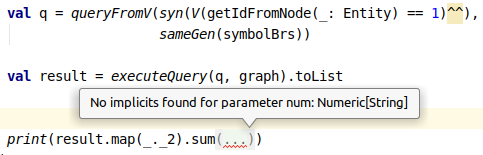
\includegraphics[width=0.48\textwidth]{pictures/image.png}
   \caption{Error notification in a query in IDEA IDE}
   \label{fig:types}
\end{figure}

\underline{\textbf{IDE Support.}}
Since you can use IDE for development, you get all features for query development, such as syntax highlighting, code navigation, autocompletion, without any additional effort.
An example of autocompletion suggestions for a vertex is presented in figure~\ref{fig:autocompletion}.

\begin{figure}[ht]
    \centering
    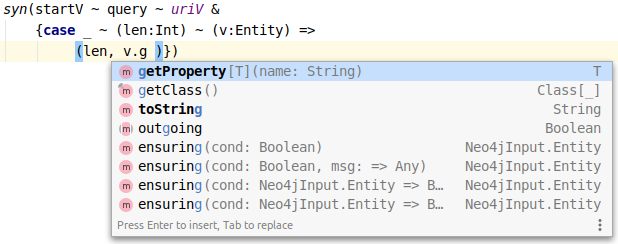
\includegraphics[width=0.48\textwidth]{pictures/image1.png}
    \caption{Query auto-completion in IDEA IDE}
    \label{fig:autocompletion}
\end{figure}
